\documentclass[12pt]{article}
 \usepackage[margin=1in]{geometry} 
\usepackage{amsmath,amsthm,amssymb,amsfonts}
\usepackage{graphics} 
\usepackage[dvipdfmx]{graphicx}

\newcommand{\N}{\mathbb{N}}
\newcommand{\Z}{\mathbb{Z}}
 
\newenvironment{problem}[2][Problem]{\begin{trivlist}
\item[\hskip \labelsep {\bfseries #1}\hskip \labelsep {\bfseries #2.}]}{\end{trivlist}}
%If you want to title your bold things something different just make another thing exactly like this but replace "problem" with the name of the thing you want, like theorem or lemma or whatever
 
\begin{document}
 
%\renewcommand{\qedsymbol}{\filledbox}
%Good resources for looking up how to do stuff:
%Binary operators: http://www.access2science.com/latex/Binary.html
%General help: http://en.wikibooks.org/wiki/LaTeX/Mathematics
%Or just google stuff
 
\title{HW 2}
\author{Motoaki Takahashi}
\maketitle
\section{Question 1}
$D_{A}=D_{B}=\frac{e}{1+2e}\approx0.4223.$

\section{Question 2}
The initial guess for the prices are $p=(1, 1)$, the initial Jacobian is the $2\times 2$ unit matrix, the predetermined tolerance is $10^{-6}$.\par
The iteration is converged, and the equilibrium prices are $(1.5989, 1.5989)$. This calculation takes 0.013 seconds.


\section{Question 3}
The Secant method is applied to get the price of one firm given the price of the other firm and the quality vector. This process is iterated along the way of Gauss-Seidel. \par
This way yields the same pricing equilibrium as Broyden method in Question 2. This calculation takes 0.039 seconds, three times as long as Broyden method in Question 2.

\section{Question 4}
Now we iteratively substitute the price of the previous step, $p^{t}$, into $p^{t+1}=\frac{1}{1-D(p^{t})}$. This iteration converges at the 12th step, and yields the same pricing equilibrium as Questions 2 and 3. This takes 0.007 seconds, much shorter than the Broyden method and the Gauss-Seidel (and Secant) method.

\section{Question 5}
Using Broyden method, I calculate the pricing equilibria for $q_{B}=0:0.2:3$.\\
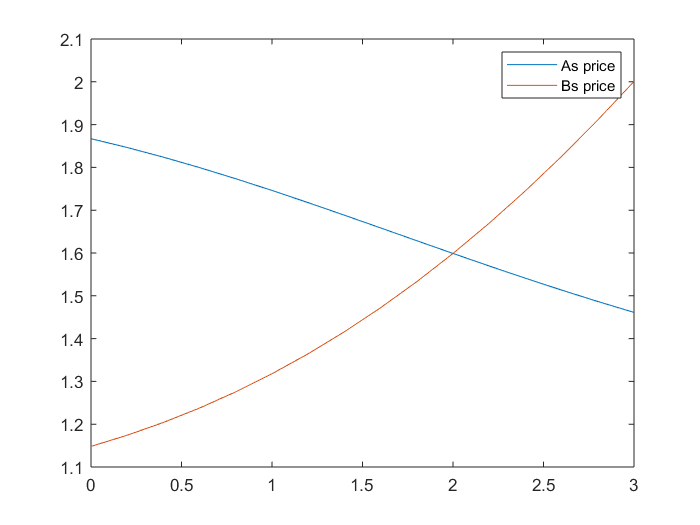
\includegraphics{price.png}\\
The above figure shows the pricing equilibria for various qualities of firm B's product. The horizontal axis is the quality of firm B product, and the vertical axis is the price level. 


\section{Code}
The following is copied from HW2.m.
\begin{tiny}
\begin{verbatim}
% HW2 for Econ 512 Empirical Methods
% Motoaki Takahashi

clear
diary hw2.out

%% Question 1
disp('Question 1')

% Define the quality vector (2 by 1)
q = [2; 2];

p = [1; 1];

demand(p, q)


%% Question 2
disp('Question 2')



% Refer to the function demand, demand.m, which returns the 2 by 1 demand vector for
% a 2 by 1 price vector and a 2 by 1 quality vector

% eqn.m defines the "left-hand side" of the equation of interest.
% That is, we want to get the value p that solves eqn(p, q)=0 for given
% quality q.

% We are interested in eqn(p,q)=0 for q = [2; 2]. Name this function
% eqn_22.
eqn_22 = @(p) eqn(p,q);

% I follow and quote the code for Broyden method in the lecture note.
% myJac.m is taken from the lecture notes.

% the initial values for the equlibrium prices
p = [1; 1];

fVal = eqn_22(p)

iJac = eye(size(p,1));
% the Broyden iterations

tic
maxit = 100;
tol = 1e-6;
for iter = 1:maxit
    fnorm = norm(fVal);
    fprintf('iter %d: p(1) = %f, p(2) = %f, norm(f(x)) = %.8f\n', iter, p(1), p(2), norm(fVal));
    if norm(fVal) < tol
        break
    end
    d = - (iJac * fVal);
    p = p+d;
    fOld = fVal;
    fVal = eqn_22(p);
    u = iJac*(fVal - fOld);
    iJac = iJac + ( (d - u) * (d'*iJac) )/ (d'*u);
end
toc

%% Question 3
disp('Question 3')

p = [1; 1];
pOld = [0;0];

tic
maxit = 100;
tol = 1e-6;

for iter = 1:maxit;
    if eqn_22(p)<tol
        fprintf('Converged: iter %d: p(1) = %f, p(2) = %f, norm(f(x)) = %.8f\n', iter, p(1), p(2), norm(eqn_22(p)));
        break
    end
    
    % Secant iteration
    
    eqn_A = @(pa) eqn_f([pa; p(2,1)], q, 1);
    
    % Secant for firm A
    pa = p(1, 1);
    paOld = pOld(1,1);
    fOld = eqn_A(paOld);
    
    tolA = 1e-8;
    for iter =1:maxit
    fVal = eqn_A(pa);
    fprintf('iter %d: pa = %.8f, f(x) = %.8f\n', iter, pa, fVal);
    if abs(fVal) < tolA
        break
    else
        paNew = pa - ( (pa - paOld) / (fVal - fOld) )* fVal;
        paOld = pa;
        pa = paNew;
        fOld = fVal;
    end
    end
    
    % Secant for firm B
    eqn_B = @(pb) eqn_f([pa; pb], q, 2);
    pb = p(2, 1);
    pbOld =  pOld(2,1);
    fOld = eqn_B(pbOld);
    
    for iter =1:maxit
    fVal = eqn_B(pb);
    fprintf('iter %d: pb = %.8f, f(x) = %.8f\n', iter, pb, fVal);
    if abs(fVal) < tolA
        break
    else
        pbNew = pb - ( (pb - pbOld) / (fVal - fOld) )* fVal;
        pbOld = pb;
        pb = pbNew;
        fOld = fVal;
    end
    p=[pa; pb]
    end
    
    
end
toc

%% Question 4
disp('Question 4')


%initial guess for p
p = [1; 1];

tic
maxit = 100;
tol = 1e-6;
for iter = 1:maxit
    pnew = ones(2,1)./(ones(2,1)-demand(p, q));
    fprintf('iter %d: p(1) = %f, p(2) = %f, norm(p-pnew) = %.8f\n', iter, p(1), p(2), norm(p-pnew));
    if norm(p-pnew) < tol
        fprintf('Converged: iter %d: p(1) = %f, p(2) = %f, norm(p-pnew) = %.8f\n', iter, p(1), p(2), norm(p-pnew));
        break
    end
    p = pnew;
end
toc
p


%% Question 5
disp('Question 5')

% the range of B's qualities
qb = 0:0.2:3;
qmatrix = [2*ones(1,length(qb));qb];
pmatrix = ones(2, length(qb));

% Solve the equilibrium price vector for each element in qb by Broyden
% method.

maxit = 100;
tol = 1e-6;
for it=1:length(qb);
    eqn_in_loop = @(pk) eqn(pk,qmatrix([1,size(qmatrix,1)],it));
    p = pmatrix([1,size(pmatrix,1)],it);
    fVal = eqn_in_loop(p);
    iJac = eye(size(p,1));
    
    for iter = 1:maxit
    fnorm = norm(fVal);
    fprintf('iter %d: p(1) = %f, p(2) = %f, norm(f(x)) = %.8f\n', iter, p(1), p(2), norm(fVal));
    if norm(fVal) < tol
        break
    end
    d = - (iJac * fVal);
    p = p+d;
    fOld = fVal;
    fVal = eqn_in_loop(p);
    u = iJac*(fVal - fOld);
    iJac = iJac + ( (d - u) * (d'*iJac) )/ (d'*u);
    end
    pmatrix([1,size(p,1)],it) = p;
end

pmatrix

plot(qmatrix(2, [1:size(qmatrix, 2)]), pmatrix(1, [1:size(pmatrix,2)]), qmatrix(2, [1:size(qmatrix, 2)]), pmatrix(2, [1:size(pmatrix,2)]))
legend('As price', 'Bs price')

diary off
\end{verbatim}
\end{tiny}
\section{Output}
The following is copied from HW2.out, which is the diary file for HW2.m.
\begin{tiny}
\begin{verbatim}
Question 1

ans =

    0.4223
    0.4223

Question 2

fVal =

    0.4223
    0.4223

iter 1: p(1) = 1.000000, p(2) = 1.000000, norm(f(x)) = 0.59724897
iter 2: p(1) = 0.577681, p(2) = 0.577681, norm(f(x)) = 0.96177748
iter 3: p(1) = 1.691933, p(2) = 1.691933, norm(f(x)) = 0.10363413
iter 4: p(1) = 1.583549, p(2) = 1.583549, norm(f(x)) = 0.01684145
iter 5: p(1) = 1.598700, p(2) = 1.598700, norm(f(x)) = 0.00026551
iter 6: p(1) = 1.598942, p(2) = 1.598942, norm(f(x)) = 0.00000069
Elapsed time is 0.013084 seconds.
Question 3
iter 1: pa = 1.00000000, f(x) = 0.42231880
iter 2: pa = 1.73105858, f(x) = -0.28043416
iter 3: pa = 1.43932904, f(x) = 0.02162624
iter 4: pa = 1.46021564, f(x) = 0.00081441
iter 5: pa = 1.46103297, f(x) = -0.00000282
iter 6: pa = 1.46103015, f(x) = 0.00000000
iter 1: pb = 1.00000000, f(x) = 0.50037200

p =

    1.4610
    2.0015

iter 2: pb = 2.00148911, f(x) = -0.46320622

p =

    1.4610
    1.5201

iter 3: pb = 1.52005857, f(x) = 0.04720684

p =

    1.4610
    1.5646

iter 4: pb = 1.56458488, f(x) = 0.00309533

p =

    1.4610
    1.5677

iter 5: pb = 1.56770933, f(x) = -0.00002737

p =

    1.4610
    1.5677

iter 6: pb = 1.56768194, f(x) = 0.00000002

p =

    1.4610
    1.5677

iter 7: pb = 1.56768196, f(x) = 0.00000000
iter 1: pa = 1.46103015, f(x) = 0.12757573
iter 2: pa = 1.67467849, f(x) = -0.08400995
iter 3: pa = 1.58984956, f(x) = 0.00206032
iter 4: pa = 1.59188017, f(x) = 0.00003051
iter 5: pa = 1.59191069, f(x) = -0.00000001
iter 6: pa = 1.59191068, f(x) = 0.00000000
iter 1: pb = 1.56768196, f(x) = 0.02951535

p =

    1.5919
    1.6154

iter 2: pb = 1.61535986, f(x) = -0.01805664

p =

    1.5919
    1.5973

iter 3: pb = 1.59726302, f(x) = 0.00010044

p =

    1.5919
    1.5974

iter 4: pb = 1.59736312, f(x) = 0.00000034

p =

    1.5919
    1.5974

iter 5: pb = 1.59736346, f(x) = -0.00000000
iter 1: pa = 1.59191068, f(x) = 0.00666865
iter 2: pa = 1.60259784, f(x) = -0.00401316
iter 3: pa = 1.59858267, f(x) = 0.00000502
iter 4: pa = 1.59858769, f(x) = 0.00000000
iter 1: pb = 1.59736346, f(x) = 0.00149852

p =

    1.5986
    1.5998

iter 2: pb = 1.59976073, f(x) = -0.00089848

p =

    1.5986
    1.5989

iter 3: pb = 1.59886215, f(x) = 0.00000025

p =

    1.5986
    1.5989

iter 4: pb = 1.59886240, f(x) = 0.00000000
iter 1: pa = 1.59858769, f(x) = 0.00033632
iter 2: pa = 1.59912551, f(x) = -0.00020149
iter 3: pa = 1.59892402, f(x) = 0.00000001
iter 4: pa = 1.59892403, f(x) = 0.00000000
iter 1: pb = 1.59886240, f(x) = 0.00007546

p =

    1.5989
    1.5990

iter 2: pb = 1.59898306, f(x) = -0.00004520

p =

    1.5989
    1.5989

iter 3: pb = 1.59893786, f(x) = 0.00000000
iter 1: pa = 1.59892403, f(x) = 0.00001693
iter 2: pa = 1.59895111, f(x) = -0.00001014
iter 3: pa = 1.59894096, f(x) = 0.00000000
iter 1: pb = 1.59893786, f(x) = 0.00000380

p =

    1.5989
    1.5989

iter 2: pb = 1.59894394, f(x) = -0.00000228

p =

    1.5989
    1.5989

iter 3: pb = 1.59894166, f(x) = 0.00000000
Converged: iter 6: p(1) = 1.598941, p(2) = 1.598942, norm(f(x)) = 0.00000085
Elapsed time is 0.039062 seconds.
Question 4
iter 1: p(1) = 1.000000, p(2) = 1.000000, norm(p-pnew) = 1.03387296
iter 2: p(1) = 1.731059, p(2) = 1.731059, norm(p-pnew) = 0.23225003
iter 3: p(1) = 1.566833, p(2) = 1.566833, norm(p-pnew) = 0.05628097
iter 4: p(1) = 1.606630, p(2) = 1.606630, norm(p-pnew) = 0.01348578
iter 5: p(1) = 1.597094, p(2) = 1.597094, norm(p-pnew) = 0.00324129
iter 6: p(1) = 1.599386, p(2) = 1.599386, norm(p-pnew) = 0.00077848
iter 7: p(1) = 1.598835, p(2) = 1.598835, norm(p-pnew) = 0.00018701
iter 8: p(1) = 1.598967, p(2) = 1.598967, norm(p-pnew) = 0.00004492
iter 9: p(1) = 1.598936, p(2) = 1.598936, norm(p-pnew) = 0.00001079
iter 10: p(1) = 1.598943, p(2) = 1.598943, norm(p-pnew) = 0.00000259
iter 11: p(1) = 1.598942, p(2) = 1.598942, norm(p-pnew) = 0.00000062
Converged: iter 11: p(1) = 1.598942, p(2) = 1.598942, norm(p-pnew) = 0.00000062
Elapsed time is 0.007225 seconds.

p =

    1.5989
    1.5989

Question 5
iter 1: p(1) = 1.000000, p(2) = 1.000000, norm(f(x)) = 0.67130547
iter 2: p(1) = 0.334759, p(2) = 0.909969, norm(f(x)) = 0.94101885
iter 3: p(1) = 2.650635, p(2) = 1.270590, norm(f(x)) = 0.88637593
iter 4: p(1) = 1.532741, p(2) = 1.063125, norm(f(x)) = 0.30514496
iter 5: p(1) = 1.823049, p(2) = 1.088974, norm(f(x)) = 0.06700035
iter 6: p(1) = 1.881497, p(2) = 1.037976, norm(f(x)) = 0.11360662
iter 7: p(1) = 0.006356, p(2) = 44.711965, norm(f(x)) = 43.72338480
iter 8: p(1) = 1.855605, p(2) = 1.125652, norm(f(x)) = 0.02339283
iter 9: p(1) = 1.862734, p(2) = 1.155634, norm(f(x)) = 0.00940052
iter 10: p(1) = 1.867036, p(2) = 1.152519, norm(f(x)) = 0.00446236
iter 11: p(1) = 1.867095, p(2) = 1.146382, norm(f(x)) = 0.00172462
iter 12: p(1) = 1.867082, p(2) = 1.148094, norm(f(x)) = 0.00000041
iter 1: p(1) = 1.000000, p(2) = 1.000000, norm(f(x)) = 0.66109061
iter 2: p(1) = 0.347760, p(2) = 0.892185, norm(f(x)) = 0.93865926
iter 3: p(1) = 2.546469, p(2) = 1.307616, norm(f(x)) = 0.77853770
iter 4: p(1) = 1.556479, p(2) = 1.085069, norm(f(x)) = 0.26804064
iter 5: p(1) = 1.814960, p(2) = 1.114044, norm(f(x)) = 0.06213473
iter 6: p(1) = 1.862368, p(2) = 1.061114, norm(f(x)) = 0.11751746
iter 7: p(1) = 1.831351, p(2) = 1.432544, norm(f(x)) = 0.26752569
iter 8: p(1) = 1.845320, p(2) = 1.164626, norm(f(x)) = 0.00954947
iter 9: p(1) = 1.846210, p(2) = 1.175387, norm(f(x)) = 0.00119766
iter 10: p(1) = 1.846435, p(2) = 1.174536, norm(f(x)) = 0.00026988
iter 11: p(1) = 1.846457, p(2) = 1.174222, norm(f(x)) = 0.00005104
iter 12: p(1) = 1.846454, p(2) = 1.174272, norm(f(x)) = 0.00000005
iter 1: p(1) = 1.000000, p(2) = 1.000000, norm(f(x)) = 0.64988735
iter 2: p(1) = 0.362966, p(2) = 0.871385, norm(f(x)) = 0.93647143
iter 3: p(1) = 2.435298, p(2) = 1.345900, norm(f(x)) = 0.66707590
iter 4: p(1) = 1.581501, p(2) = 1.114031, norm(f(x)) = 0.22730812
iter 5: p(1) = 1.804264, p(2) = 1.145374, norm(f(x)) = 0.05773656
iter 6: p(1) = 1.841925, p(2) = 1.092470, norm(f(x)) = 0.11728888
iter 7: p(1) = 1.817154, p(2) = 1.290083, norm(f(x)) = 0.08912697
iter 8: p(1) = 1.823576, p(2) = 1.199324, norm(f(x)) = 0.00475375
iter 9: p(1) = 1.823813, p(2) = 1.204527, norm(f(x)) = 0.00045953
iter 10: p(1) = 1.823881, p(2) = 1.204161, norm(f(x)) = 0.00006846
iter 11: p(1) = 1.823888, p(2) = 1.204090, norm(f(x)) = 0.00000472
iter 12: p(1) = 1.823888, p(2) = 1.204095, norm(f(x)) = 0.00000000
iter 1: p(1) = 1.000000, p(2) = 1.000000, norm(f(x)) = 0.63795069
iter 2: p(1) = 0.380604, p(2) = 0.847259, norm(f(x)) = 0.93471351
iter 3: p(1) = 2.319478, p(2) = 1.384518, norm(f(x)) = 0.55567545
iter 4: p(1) = 1.606061, p(2) = 1.151307, norm(f(x)) = 0.18449319
iter 5: p(1) = 1.790233, p(2) = 1.183716, norm(f(x)) = 0.05285544
iter 6: p(1) = 1.819803, p(2) = 1.133424, norm(f(x)) = 0.11172021
iter 7: p(1) = 1.795994, p(2) = 1.272238, norm(f(x)) = 0.03597767
iter 8: p(1) = 1.799439, p(2) = 1.235668, norm(f(x)) = 0.00216215
iter 9: p(1) = 1.799481, p(2) = 1.237975, norm(f(x)) = 0.00016334
iter 10: p(1) = 1.799506, p(2) = 1.237840, norm(f(x)) = 0.00001817
iter 11: p(1) = 1.799509, p(2) = 1.237822, norm(f(x)) = 0.00000055
iter 1: p(1) = 1.000000, p(2) = 1.000000, norm(f(x)) = 0.62572100
iter 2: p(1) = 0.400865, p(2) = 0.819544, norm(f(x)) = 0.93372547
iter 3: p(1) = 2.202166, p(2) = 1.422618, norm(f(x)) = 0.44863898
iter 4: p(1) = 1.627604, p(2) = 1.197653, norm(f(x)) = 0.14199447
iter 5: p(1) = 1.772194, p(2) = 1.229411, norm(f(x)) = 0.04634708
iter 6: p(1) = 1.795329, p(2) = 1.184804, norm(f(x)) = 0.09988463
iter 7: p(1) = 1.771687, p(2) = 1.289704, norm(f(x)) = 0.01484619
iter 8: p(1) = 1.773507, p(2) = 1.274813, norm(f(x)) = 0.00088857
iter 9: p(1) = 1.773492, p(2) = 1.275732, norm(f(x)) = 0.00004780
iter 10: p(1) = 1.773501, p(2) = 1.275692, norm(f(x)) = 0.00000414
iter 11: p(1) = 1.773502, p(2) = 1.275688, norm(f(x)) = 0.00000006
iter 1: p(1) = 1.000000, p(2) = 1.000000, norm(f(x)) = 0.61386472
iter 2: p(1) = 0.423883, p(2) = 0.788058, norm(f(x)) = 0.93391213
iter 3: p(1) = 2.087237, p(2) = 1.459713, norm(f(x)) = 0.35044672
iter 4: p(1) = 1.643045, p(2) = 1.252771, norm(f(x)) = 0.10277848
iter 5: p(1) = 1.749727, p(2) = 1.282133, norm(f(x)) = 0.03748863
iter 6: p(1) = 1.767631, p(2) = 1.246326, norm(f(x)) = 0.08161459
iter 7: p(1) = 1.745202, p(2) = 1.323463, norm(f(x)) = 0.00600251
iter 8: p(1) = 1.746129, p(2) = 1.317573, norm(f(x)) = 0.00033671
iter 9: p(1) = 1.746105, p(2) = 1.317907, norm(f(x)) = 0.00001079
iter 10: p(1) = 1.746107, p(2) = 1.317898, norm(f(x)) = 0.00000073
iter 1: p(1) = 1.000000, p(2) = 1.000000, norm(f(x)) = 0.60329372
iter 2: p(1) = 0.449705, p(2) = 0.752737, norm(f(x)) = 0.93569230
iter 3: p(1) = 1.979042, p(2) = 1.496100, norm(f(x)) = 0.26520066
iter 4: p(1) = 1.649533, p(2) = 1.314958, norm(f(x)) = 0.06970771
iter 5: p(1) = 1.722931, p(2) = 1.340673, norm(f(x)) = 0.02660767
iter 6: p(1) = 1.736067, p(2) = 1.315917, norm(f(x)) = 0.05833073
iter 7: p(1) = 1.717157, p(2) = 1.366729, norm(f(x)) = 0.00233985
iter 8: p(1) = 1.717626, p(2) = 1.364515, norm(f(x)) = 0.00011418
iter 9: p(1) = 1.717609, p(2) = 1.364622, norm(f(x)) = 0.00000177
iter 10: p(1) = 1.717609, p(2) = 1.364621, norm(f(x)) = 0.00000009
iter 1: p(1) = 1.000000, p(2) = 1.000000, norm(f(x)) = 0.59513973
iter 2: p(1) = 0.478268, p(2) = 0.713667, norm(f(x)) = 0.93940544
iter 3: p(1) = 1.882019, p(2) = 1.533333, norm(f(x)) = 0.19611705
iter 4: p(1) = 1.645560, p(2) = 1.381353, norm(f(x)) = 0.04472346
iter 5: p(1) = 1.692706, p(2) = 1.402988, norm(f(x)) = 0.01542123
iter 6: p(1) = 1.701085, p(2) = 1.389373, norm(f(x)) = 0.03397417
iter 7: p(1) = 1.688085, p(2) = 1.416739, norm(f(x)) = 0.00087223
iter 8: p(1) = 1.688327, p(2) = 1.415970, norm(f(x)) = 0.00003048
iter 9: p(1) = 1.688320, p(2) = 1.415997, norm(f(x)) = 0.00000033
iter 1: p(1) = 1.000000, p(2) = 1.000000, norm(f(x)) = 0.59065896
iter 2: p(1) = 0.509371, p(2) = 0.671121, norm(f(x)) = 0.94518427
iter 3: p(1) = 1.800152, p(2) = 1.574645, norm(f(x)) = 0.14530084
iter 4: p(1) = 1.631746, p(2) = 1.449023, norm(f(x)) = 0.02830480
iter 5: p(1) = 1.660835, p(2) = 1.466895, norm(f(x)) = 0.00658847
iter 6: p(1) = 1.664982, p(2) = 1.461598, norm(f(x)) = 0.01456627
iter 7: p(1) = 1.658421, p(2) = 1.472415, norm(f(x)) = 0.00037177
iter 8: p(1) = 1.658568, p(2) = 1.472127, norm(f(x)) = 0.00000608
iter 9: p(1) = 1.658566, p(2) = 1.472132, norm(f(x)) = 0.00000014
iter 1: p(1) = 1.000000, p(2) = 1.000000, norm(f(x)) = 0.59105579
iter 2: p(1) = 0.542671, p(2) = 0.625571, norm(f(x)) = 0.95283289
iter 3: p(1) = 1.736348, p(2) = 1.625184, norm(f(x)) = 0.11403045
iter 4: p(1) = 1.610393, p(2) = 1.516365, norm(f(x)) = 0.01948723
iter 5: p(1) = 1.629339, p(2) = 1.531544, norm(f(x)) = 0.00196969
iter 6: p(1) = 1.630882, p(2) = 1.530258, norm(f(x)) = 0.00434485
iter 7: p(1) = 1.628487, p(2) = 1.533342, norm(f(x)) = 0.00036797
iter 8: p(1) = 1.628672, p(2) = 1.533098, norm(f(x)) = 0.00000185
iter 9: p(1) = 1.628671, p(2) = 1.533099, norm(f(x)) = 0.00000012
iter 1: p(1) = 1.000000, p(2) = 1.000000, norm(f(x)) = 0.59724897
iter 2: p(1) = 0.577681, p(2) = 0.577681, norm(f(x)) = 0.96177748
iter 3: p(1) = 1.691933, p(2) = 1.691933, norm(f(x)) = 0.10363413
iter 4: p(1) = 1.583549, p(2) = 1.583549, norm(f(x)) = 0.01684145
iter 5: p(1) = 1.598700, p(2) = 1.598700, norm(f(x)) = 0.00026551
iter 6: p(1) = 1.598942, p(2) = 1.598942, norm(f(x)) = 0.00000069
iter 1: p(1) = 1.000000, p(2) = 1.000000, norm(f(x)) = 0.60964829
iter 2: p(1) = 0.613793, p(2) = 0.528285, norm(f(x)) = 0.97114918
iter 3: p(1) = 1.666444, p(2) = 1.783380, norm(f(x)) = 0.11679881
iter 4: p(1) = 1.550669, p(2) = 1.650946, norm(f(x)) = 0.02032101
iter 5: p(1) = 1.565822, p(2) = 1.672032, norm(f(x)) = 0.00547242
iter 6: p(1) = 1.561692, p(2) = 1.675832, norm(f(x)) = 0.01238050
iter 7: p(1) = 1.569823, p(2) = 1.669566, norm(f(x)) = 0.00024027
iter 8: p(1) = 1.569655, p(2) = 1.669675, norm(f(x)) = 0.00000441
iter 9: p(1) = 1.569658, p(2) = 1.669674, norm(f(x)) = 0.00000008
iter 1: p(1) = 1.000000, p(2) = 1.000000, norm(f(x)) = 0.62802969
iter 2: p(1) = 0.650313, p(2) = 0.478329, norm(f(x)) = 0.97999663
iter 3: p(1) = 1.657841, p(2) = 1.909123, norm(f(x)) = 0.15916585
iter 4: p(1) = 1.507671, p(2) = 1.715967, norm(f(x)) = 0.03346918
iter 5: p(1) = 1.524045, p(2) = 1.754104, norm(f(x)) = 0.02319773
iter 6: p(1) = 1.502465, p(2) = 1.768176, norm(f(x)) = 0.05478869
iter 7: p(1) = 1.541831, p(2) = 1.745121, norm(f(x)) = 0.00088257
iter 8: p(1) = 1.540986, p(2) = 1.745313, norm(f(x)) = 0.00009936
iter 9: p(1) = 1.541059, p(2) = 1.745282, norm(f(x)) = 0.00000497
iter 10: p(1) = 1.541062, p(2) = 1.745280, norm(f(x)) = 0.00000018
iter 1: p(1) = 1.000000, p(2) = 1.000000, norm(f(x)) = 0.65156434
iter 2: p(1) = 0.686520, p(2) = 0.428803, norm(f(x)) = 0.98754150
iter 3: p(1) = 1.663055, p(2) = 2.079683, norm(f(x)) = 0.24119059
iter 4: p(1) = 1.448499, p(2) = 1.770207, norm(f(x)) = 0.06337439
iter 5: p(1) = 1.466239, p(2) = 1.843476, norm(f(x)) = 0.05961807
iter 6: p(1) = 1.400537, p(2) = 1.876455, norm(f(x)) = 0.14805240
iter 7: p(1) = 1.517460, p(2) = 1.825849, norm(f(x)) = 0.00420027
iter 8: p(1) = 1.512573, p(2) = 1.825920, norm(f(x)) = 0.00093168
iter 9: p(1) = 1.513304, p(2) = 1.825744, norm(f(x)) = 0.00007112
iter 10: p(1) = 1.513353, p(2) = 1.825720, norm(f(x)) = 0.00000486
iter 11: p(1) = 1.513357, p(2) = 1.825718, norm(f(x)) = 0.00000002
iter 1: p(1) = 1.000000, p(2) = 1.000000, norm(f(x)) = 0.67898644
iter 2: p(1) = 0.721714, p(2) = 0.380662, norm(f(x)) = 0.99335594
iter 3: p(1) = 1.678625, p(2) = 2.306649, norm(f(x)) = 0.38018033
iter 4: p(1) = 1.368869, p(2) = 1.799274, norm(f(x)) = 0.11746386
iter 5: p(1) = 1.388766, p(2) = 1.933917, norm(f(x)) = 0.11451593
iter 6: p(1) = 1.254100, p(2) = 1.988509, norm(f(x)) = 0.28410904
iter 7: p(1) = 1.502615, p(2) = 1.913261, norm(f(x)) = 0.01559411
iter 8: p(1) = 1.482794, p(2) = 1.911184, norm(f(x)) = 0.00421488
iter 9: p(1) = 1.486506, p(2) = 1.910995, norm(f(x)) = 0.00025083
iter 10: p(1) = 1.486684, p(2) = 1.910930, norm(f(x)) = 0.00002354
iter 11: p(1) = 1.486702, p(2) = 1.910923, norm(f(x)) = 0.00000043
iter 1: p(1) = 1.000000, p(2) = 1.000000, norm(f(x)) = 0.70882830
iter 2: p(1) = 0.755272, p(2) = 0.334759, norm(f(x)) = 0.99739228
iter 3: p(1) = 1.701225, p(2) = 2.603113, norm(f(x)) = 0.60265087
iter 4: p(1) = 1.270496, p(2) = 1.787015, norm(f(x)) = 0.20195475
iter 5: p(1) = 1.292943, p(2) = 2.015133, norm(f(x)) = 0.18053729
iter 6: p(1) = 1.079898, p(2) = 2.092045, norm(f(x)) = 0.43579094
iter 7: p(1) = 1.511758, p(2) = 2.010778, norm(f(x)) = 0.04895916
iter 8: p(1) = 1.446846, p(2) = 1.999359, norm(f(x)) = 0.01434528
iter 9: p(1) = 1.460781, p(2) = 2.000847, norm(f(x)) = 0.00047982
iter 10: p(1) = 1.461190, p(2) = 2.000812, norm(f(x)) = 0.00003233
iter 11: p(1) = 1.461213, p(2) = 2.000803, norm(f(x)) = 0.00000280
iter 12: p(1) = 1.461215, p(2) = 2.000803, norm(f(x)) = 0.00000003

pmatrix =

    1.8671    1.8465    1.8239    1.7995    1.7735    1.7461    1.7176    1.6883    1.6586    1.6287    1.5989    1.5697    1.5411    1.5134    1.4867    1.4612
    1.1481    1.1743    1.2041    1.2378    1.2757    1.3179    1.3646    1.4160    1.4721    1.5331    1.5989    1.6697    1.7453    1.8257    1.9109    2.0008

\end{verbatim}
\end{tiny}
\end{document}

